
\documentclass{article}

\usepackage{graphicx}
\usepackage{hyperref}
\usepackage{amsmath}
\usepackage{algorithm}
%\usepackage{algorithmic}
\usepackage{algpseudocode}
\usepackage{subcaption}
\usepackage{booktabs}

\usepackage[
  paper  = letterpaper,
  left   = 1.25in,
  right  = 1.25in,
  top    = 1.0in,
  bottom = 1.0in,
  ]{geometry}
\usepackage{setspace}




\graphicspath{{images/}}

\title{Hidden enemy detecting using bayes inference}

\author{yueyi zhuo(2014060843)}

\date{2018}

\begin{document}

\maketitle

\begin{abstract}

Assuming a location which have samll distance to two conflict side have more probability cause a battle,
how do we infer the location of enemy if we can only observe the locations of ally and battle? The latent
variable inference problem requiere a decent front probability model and a effiecent way to run the 
inference. In this work, a battle model is introduced and a bayes inference framework based on pytorch 
is developed to complete the inference task including point and movement detection and 
exist probability estimation with different prior and various initialization value setting.
A case study about The battle of Gettysburg is included to show the overview of the content covered by the paper.

\end{abstract}

\section{Introduction}

In real warfare, you can't observe enemy units even ally unit as RTS or classic board wargame way.
The only thing you can rely are complex and confusing even self-contradiction information and misinformation.
There're a lot of example, that general misunderstand information and may be defeated due to this. 
Bing Sun manipulated field kitchen of his army to trick his opponent, General McClellan reject to attack
due to "peace gun"(fake gun instrument) seted by south rebel, lossing oppotunity to beat rebel down.

Unfortunately, current military decision similation program, such as "classic" wargame Figure~\ref{fig:hps} and somewhat 
"serious" RTS, tend to capture more "macro" aspect and simplify the reconnaissance and 
information modeling aspect into a unaccepted level.

\begin{figure}[h]
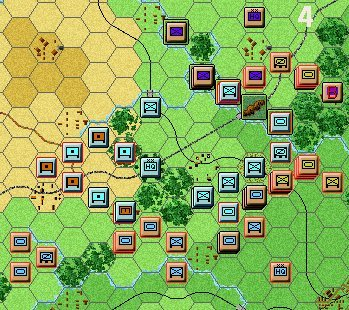
\includegraphics[width=0.6\linewidth]{SmolenskR4.jpg}
\caption{This figure show the reconnassance treatment of Smolensk' 41, 
a classic hex wargame developed by HPS.
Units can only be observed wholly or can't be observed. }
\label{fig:hps}
\end{figure}

Though we can read the oob(order of battle) as Figure~\ref{fig:metz} from map of battle, but it's obvious that those marks are 
placed in there using post Liang Zhuge information. In real time battle field, you can only hear where
be attacked and where observe the trace of enemy (instead of unit detail id or somewhat strange quatity
information), and some of them may be wrong and some of them may be released by enemy to confuse you.
The movement of Jackson in valley campaign is a vivid example about how the fake information intentionally
made by oppnent weak the strength of army.

\begin{figure}[h]
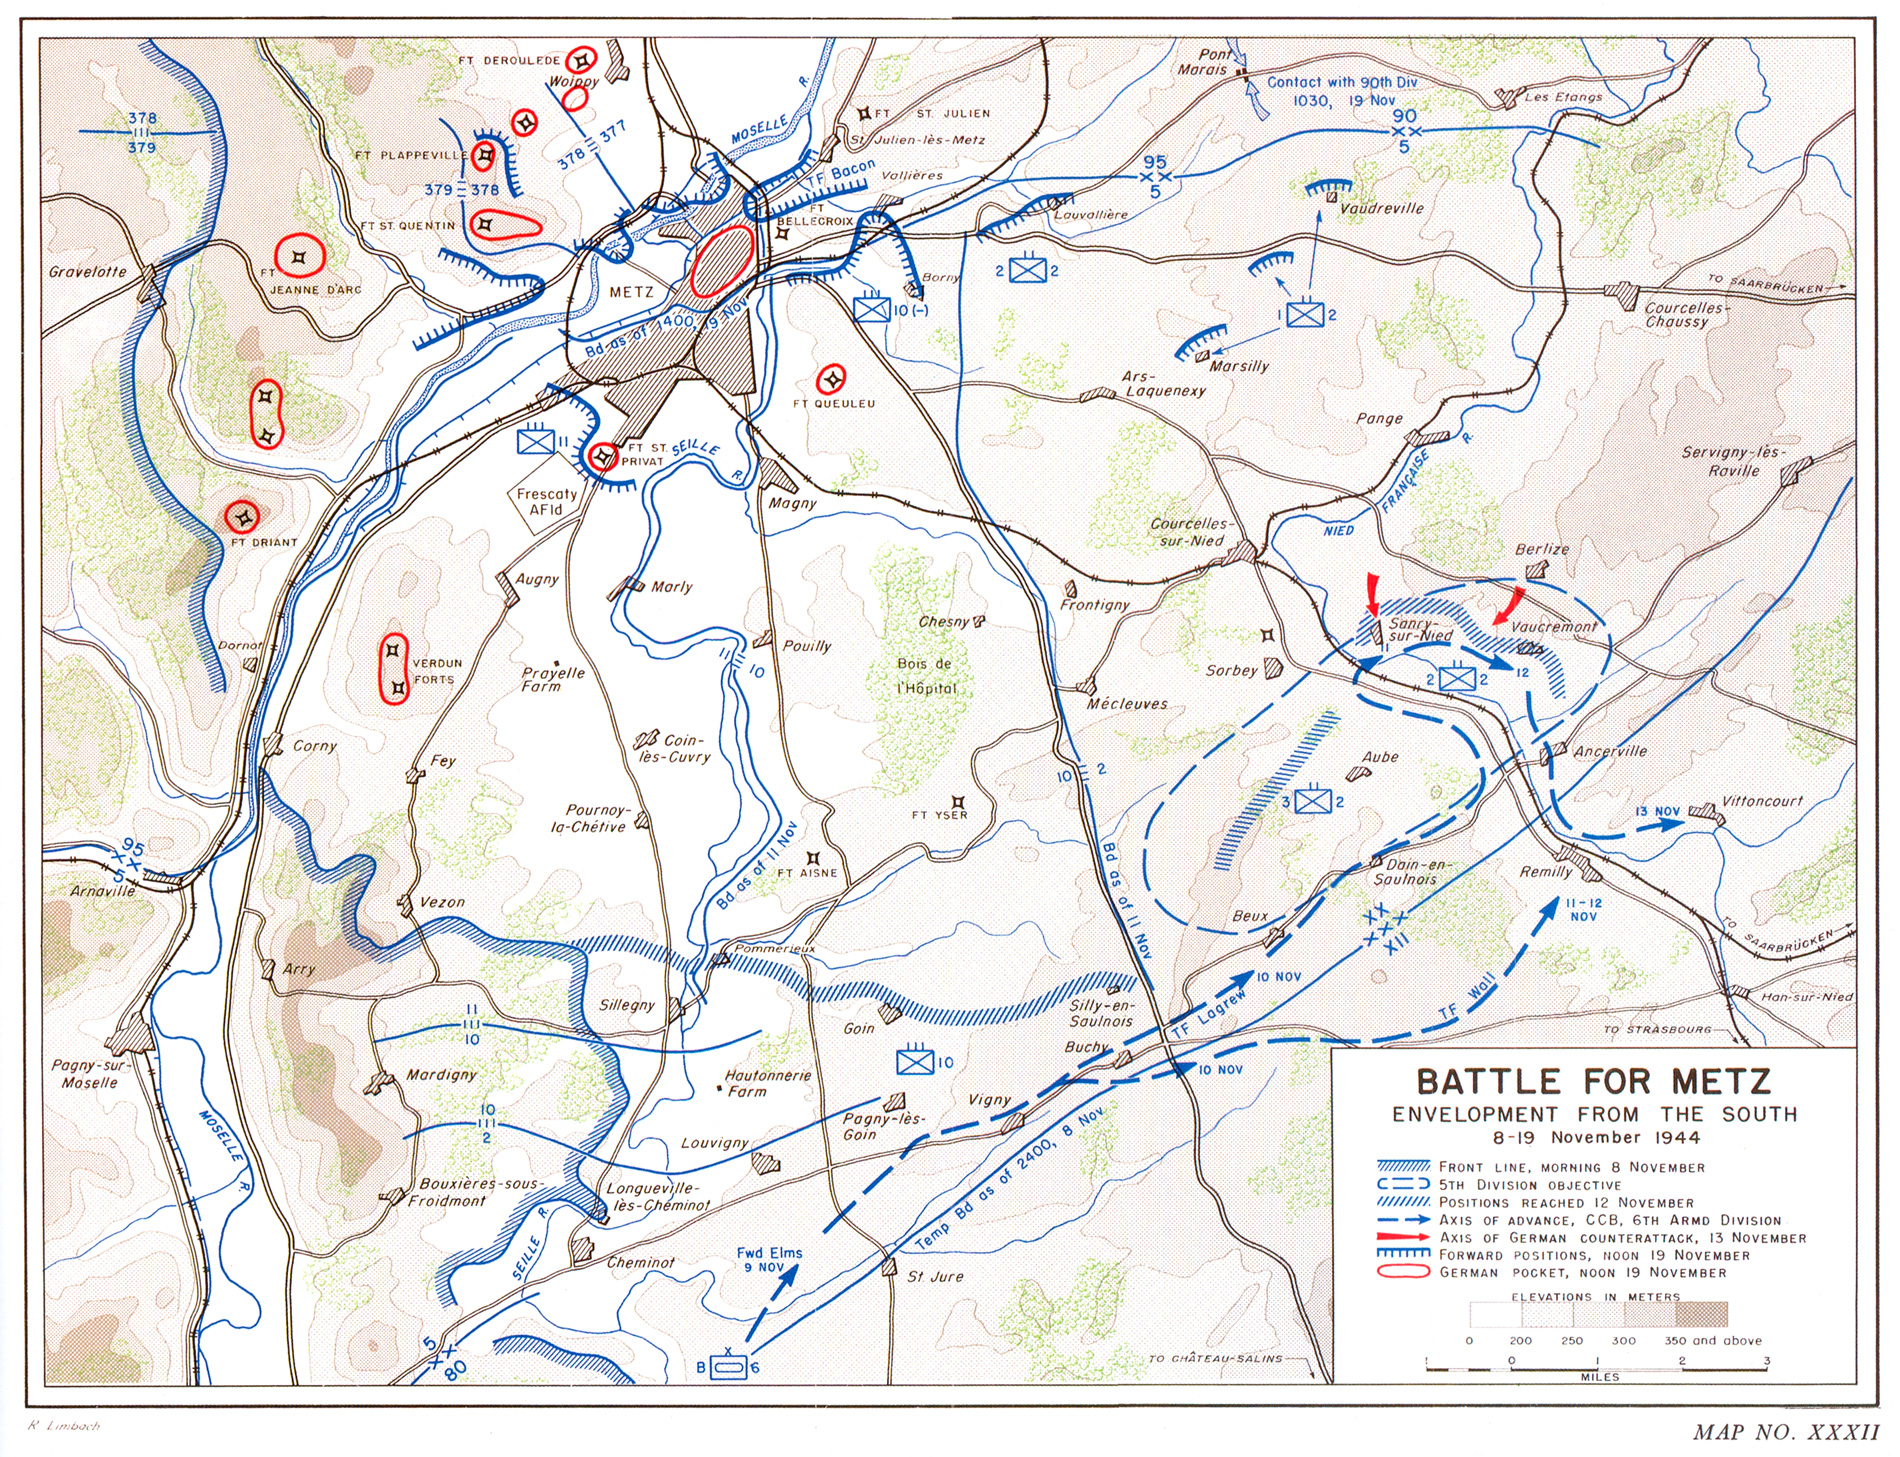
\includegraphics[width=0.6\linewidth]{metz.jpg}
\caption{The map of battle of Metz, showing oob that can't be observed in real time battlefied. }
\label{fig:metz}
\end{figure}


Some work were made to solve this problem 
\cite{hostetler2012inferring} \cite{vsmejkal2016integrating} \cite{touhou}.
Since they filter small part of information from replay file, they made a case that enemy can not be 
seen in that direct way, then they proposed according probability model to rebuild real situation.
They're good try, but not real demand for most of case. The paper we
\footnote{Though the paper only have a writer, 
but "we" seems a traditional and kind pronoun for such paper. 
In following content, both "we" and "I" will be used to represent the writer.} 
wrote will deal the problem in a more direct way. 
A coordinate based position and movement detecting method is present in this paper.

\section{Building a proper forward model}


In forward model, a process that can give probility of number of battles and the mass in support space 
is required. For example, given ally and ememy location setting as Figure~\ref{fig:stateNoBattle}.

\begin{figure}[h]
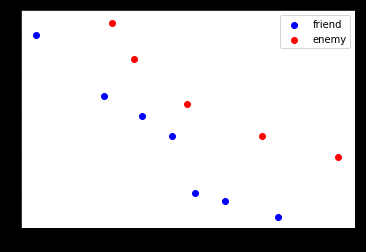
\includegraphics{state_no_battle.png}
\caption{Ally and enemy setting}
\label{fig:stateNoBattle}
\end{figure}

\subsection{A basic setting}

Suppose the the number of battle is 10, we can model the 10 battles are indepently drawn from below 
distribution:

$$
P(x,y) \propto \max_i p^A_{i}(x,y) \max_j p^E_{j} (x,y)
$$

Where $p^A_{i}(x,y)$ indicate the probability density "released" from of i’st ally unit,
$p^E_{j}$ indicate same thing from j’st enemy unit. And the density is defined by:

$$
P^S_i(x,y) \propto \exp(-\frac{1}{2}((x-x^S_i)^2 + (y-y^S_i)^2))
$$

Where the probability in $(x,y)$ released from i'th unit of S side(enemy or ally). 
So we can rewrite above formula as: 

$$
P(x,y) \propto \exp(-\frac{1}{2}((x-x_{nearst(x,y)})^2 + (y-y_{nearst(x,y)})^2))
$$

Where $nearst(x,y)$ indicate the the unit(enemy or ally) which is nearest to (x,y).

This means the non-normalized probability is only subject to the nearest two conflict units’s distance, 
though the assumption don’t have abundant meaning. 
It capture something crucial but have obvious weakness such as independent hypothesis, lately the 
model will be adujusted mutiple times to fix this and other problems. Anyway, the probability
 can be computed and visualized as contour Figure~\ref{fig:stateNoBattleProb}.

\begin{figure}[h]
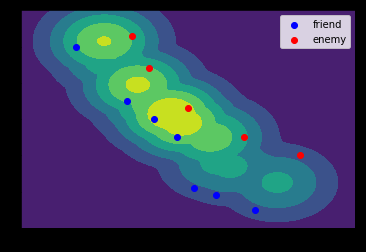
\includegraphics{state_no_battle_prob.png}
\caption{Battle density distribution}
\label{fig:stateNoBattleProb}
\end{figure}

The probability don't have a standard shape, implying it's hard to sample. To overcome this, the "grid 
sampling" method is used. In this example, the support of density is limited to $[-1,5] \times [0,6]$
(the point on the out sideof $[-1,5] \times [0,6]$ have zero density). And $100 \times 100$ points are 
selected to build a grid approxmation. See size-reduced version in Figure~\ref{fig:gridify}.

\begin{figure}[h]
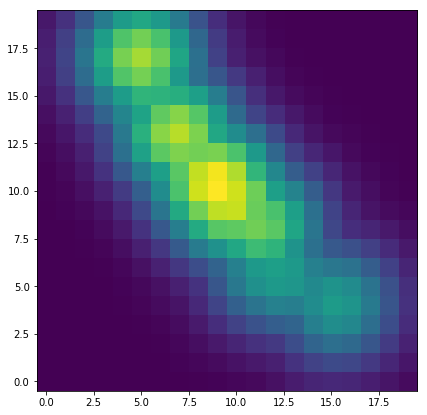
\includegraphics[width=0.6\linewidth]{gridify.png}
\caption{$25 \times 25$ discrete approxmation}
\label{fig:gridify}
\end{figure}

So firstly we draw a square in the grid according to the approximated probability, 
and then draw two uniform variable $dX \sim U(0,5-(-1)/100),dY \sim U(0,(6-0)/100)$ 
to determine the position drew by this process.

Repeating the process 10 times, we can get size 10 independent sample from the distribution as such Figure~\ref{fig:stateSampleBattle}.

\begin{figure}[h]
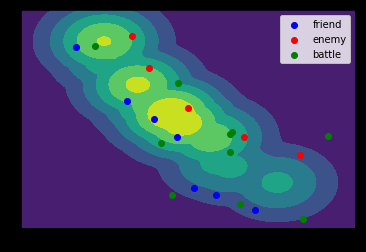
\includegraphics[width=0.6\linewidth]{state_sample_battle.png}
\caption{Ally,enemy,prob, and a sample of battle}
\label{fig:stateSampleBattle}
\end{figure}

If the positions of enemy is hidden, then we can get a instance of problem data as Figure~\ref{fig:stateNoEnemy}.

\begin{figure}[h]
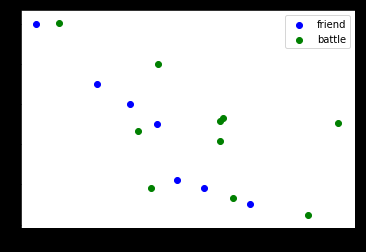
\includegraphics[width=0.6\linewidth]{state_no_enemy.png}
\caption{hide enemy}
\label{fig:stateNoEnemy}
\end{figure}

\subsection{A complex setting}

Although the distribution may satisfy our goal, but the $\min$ function will cause that gradient-based optmization
method doesn't work in those units whose is not nearest to observed battle. So we proposed another setting:

First, a classifier is used to determine the "conflict level" in every point.
Supposing a point is more likely be controled by S side 
if a unit of S side have shortest distance to it, then we can define that the more two control probability 
being close to eachother, the more conflict chance in this point. So the conflict factor is defined by:

$$
P_{\text{conflict}}(x,y) = P_\text{ally}(x,y) P_\text{enemy}(x,y)
$$

Where $P_\text{ally}(x,y)$ indicate the probability(belief) of $(x,y)$ is classified 
in ally given by classifer.

In this paper, we use naive bayes classifer as classifer since it helps gradient computation. The 
classify probability are given by:

$$
P_\text{ally}(x,y) = \frac{
N(x\mid \mu_\text{ally} ,\sigma_\text{ally}) N(y  \mid \mu_\text{ally}, \sigma_\text{ally})
}{
N(x \mid \mu_\text{ally} , \sigma_\text{ally}) N(y \mid \mu_\text{ally} , \sigma_\text{ally}) + 
N(x \mid \mu_\text{enemy} , \sigma_\text{enemy}) N(y \mid \mu_\text{enemy} , \sigma_\text{enemy})
}
$$

Where $N(x \mid \mu,\sigma)$ is normal probability density function:
$$
N(x \mid \mu,\sigma) = \frac{1}{\sqrt{2\pi \sigma^2}} \exp\left(\frac{(x-\mu)^2}{2\sigma^2}\right)
$$

The classifier parameters $\mu,\sigma$ are estimated by normal moment estimation.

There's the classify probability, see Figure~\ref{fig:naivebayes}.

\begin{figure}[h]
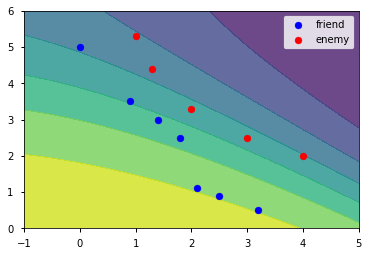
\includegraphics[width=0.6\linewidth]{naivebayes.png}
\caption{naive bayes predict probability coutour map}
\label{fig:naivebayes}
\end{figure}

Then, we define that the less the distance between point and any units(ally or enemy) be,
the more likely the point will occur a battle.

$$
P_{\text{distance}}(x,y) = \exp(-\alpha \min_{u} distance)
$$

Where $u$ means unit. $\min_u distance$ the shortest distance in all possible distance 
between coordinate of unit and $(x,y)$.

So the probability is:

$$
P(x,y) = P_{\text{conflict}}(x,y) P_{\text{distance}}(x,y) = 
P_\text{ally}(x,y) P_\text{enemy}(x,y) \exp(-\alpha \min_{u} distance)
$$

Set $\alpha=0.1$, the result can be seen as Figure~\ref{fig:combOne}:

\begin{figure}[h]
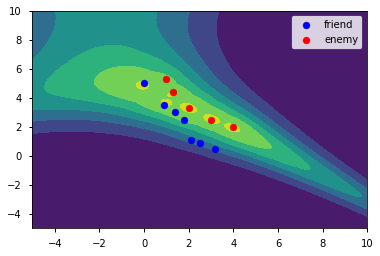
\includegraphics[width=0.6\linewidth]{comb1.png}
\caption{Combining a naive bayes classifier and a smooth distance factor}
\label{fig:combOne}
\end{figure}

The smooth probability seems good, but the sample result seems too diffused 
(Figure~\ref{fig:combTwo}) and when scale is enlarged, the problem even worsen (\ref{fig:combThree}).
Some parameters tuning are tried but not satisfy the demand. So the smooth function family are droped 
and uniform distribution is adopted. 

\begin{figure}[h]
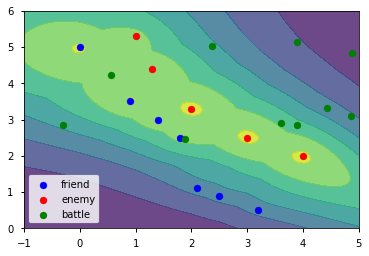
\includegraphics[width=0.6\linewidth]{comb2.png}
\caption{Too diffused sample}
\label{fig:combTwo}
\end{figure}

\begin{figure}[h]
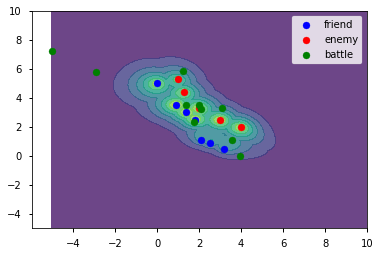
\includegraphics[width=0.6\linewidth]{comb4.png}
\caption{When extend the scale, unrational sample will present inevitably.}
\label{fig:combThree}
\end{figure}

\subsection{Selected setting}

We assign a point constant probability if it is greater than conflict threshold and less than distance 
threshold:

$$
P(x,y) \propto
\begin{cases}
1 & P_\text{ally}(x,y) (1-P_\text{ally}(x,y)) > \text{ conflict threshold and }
    \min_{u} distance < \text{conflict threshold} \\
0 & \text{otherwise}
\end{cases}
$$

Figure~\ref{fig:combFive} shows how the unrational sample point is suppressed.

\begin{figure}[h]
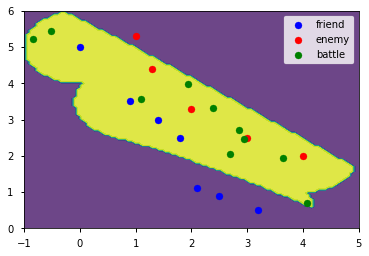
\includegraphics[width=0.6\linewidth]{comb5.png}
\caption{Forced 0 zero probability can suppress the unrational point}
\label{fig:combFive}
\end{figure}

To get gradient information to proceed optimization, rewrite the conditional jump function to "soft"
version, for example, sigmoid function $sig(x) = \frac{1}{1+\exp(-x)}$:

$$
P(x,y) \propto sig(t (P_\text{ally}(x,y) (1-P_\text{ally}(x,y)) - \theta_0)) sig(t(-\min_{u} distance + \theta_1))
$$

Where $t$ is "tense" parameter controling the shape of sigmoid, $\theta_0,\theta_1$ are threshold for
conflict level and distance. For $\theta_0=0.2,\theta_1=1.5,t = 10.0$, the result can be show in Figure~\ref{fig:combSix}.

\begin{figure}[h]
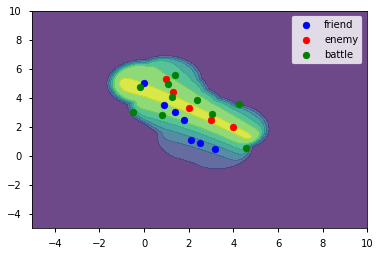
\includegraphics[width=0.6\linewidth]{comb6.png}
\caption{Selected model}
\label{fig:combSix}
\end{figure}

The model seems perfect to our demand, following article will use it.

\section{A framework and algorithms for inference}

A bayes inference framework is a programming language or a library that is made to organize the 
programming for model and inference related optmization code.

\subsection{Former inference framework}

There're a lot of inference framework such as Stan \cite{carpenter2017stan}, 
pymc\cite{patil2010pymc} and edward \cite{tran2016edward}. 
The core of them are a automated gradient computation library, 
they're stan-math, theano, tensorflow respectively. 

Nevertheless, those except stan are too weak in their ability describing complex probabiliy function.
And the compile time of stan is too long. So a light-weight bayes inference library is proposed to 
fulfill our goal. The framework is based on pytorch providing a flexible automated gradient computation lib and easy-to-use 
dynamic computation graph as Chainer.

\subsection{Inference method and algorithm introduction}

In this section, three inference method used below sections will be introduced.

\subsubsection{Maximum A Posteriori}

Maximum A Posteriori(MAP) is a estimator that maximize the likelihood function 
coporating prior information. Since the task of gradient computation is done by pytorch, 
we can only call the SGD or any other artful NN(neural net)-oriented optimizer to do standard gradient 
descent (take $loss = -likelihood \times prior$) process. See Algorithm~\ref{alg:sgd}.


\begin{algorithm}
\caption{Stochastic gradient descent}
\begin{algorithmic}[1]
\Procedure{SGD}{$\theta,lr,step$}
    \For{i in 1:step}
        \State $\nabla \gets (\nabla_\theta \log(x,\theta)|_{\theta})$
        \State $\theta \gets \theta - lr \nabla -\theta$
    \EndFor
    \State \textbf{return} $\theta$
\EndProcedure
\end{algorithmic}
\label{alg:sgd}
\end{algorithm}

\subsubsection{Variational inference}

Variational inference use simple joint distribution setting to approximate complex 
exact posterior distribution, using Kullback-Leibler(KL) diversity as optimizing target \cite{blei2017variational}. That is:

$$
KL(q||p) = E_q \left( \log \frac{q(\theta \mid \mu,\omega)}{p(\theta \mid x)} \right)
$$

Where $p(\theta \mid x)$ is exact posterior distribution. 
$q(\theta)$ is corresponding variational distribution approximating the exact one.
The family of $q(\theta)$ are usually employed as normal distribution, especially $N(\mu,\mathbf{\Sigma})$ form.
If $\mathbf{\Sigma}=\mathrm{diag}(exp(\mathbf{\omega}))$, 
that is so called meanfield setting we will see it in following content.
%$q(\theta \mid \mu,\omega)$ is corresponding variational distribution approximating the exact one
%and the $\mu,\omega=\log(\sigma)$ means the distribution is in normal family with independent variable(meanfield).
%The $\mu,\omega$ will be omited in following content.

Since it employ variational distribution $q(\theta)$ as expectation weight 
instead of exact posterior distribution,
the computation difficulty is relative reduced. But it seems too hard to deal too. So 
we turn to considering evidence lower bound(ELBO) which is lower bound for $\log p(x)$:

\begin{align*}
\log p(x) &= \log \int_\theta p(x,\theta) = \log \int_\theta p(x,\theta) \frac{q(\theta)}{q(\theta)} = \log \left( E_q \frac{p(x,\theta)}{q(\theta)} \right)  \\
          &\ge E_q (\log p(x,\theta)) - E_q(\log q(\theta)) = \mathrm{ELBO}
\end{align*}

The relation of KL diversity and ELBO can be show:

\begin{align*}
KL(q(\theta) || p(\theta \mid x)) &= E_q \log \frac{q(\theta)}{p(\theta \mid x)}  \\
                                  &= E_q \log q(\theta) - E_q \log p(\theta \mid x) \\
                                  &= E_q \log q(\theta) - E_q \log p(\theta,x) + E_q \log p(x) \\
                                  &= -(E_q \log p(\theta,x) -E_q \log q(\theta)) + \log p(x) \\
                                  &= -\mathrm{ELBO} + \log p(x)
\end{align*}

So we can maximizing ELBO to minimizing KL diversity. 
To do the optimization, the tradition variational inference method, 
Coordinate ascent variational inference (CAVI) algorithm,
require a analytic conditional expectation $E_{-j}(\log p(\theta_j \mid \mathbf{\theta}_{-j},\mathbf{x}))$. 
It's annoy when user aware that he can do sampling to
reach same goal without any of such brain exhausted requirment. 

The Automatic differentiation variational inference (ADVI) is presented by 
\cite{kucukelbir2017automatic} and \cite{kucukelbir2014fully}
to fix it. The core of the algorithm is to use random integral to approximate a hard-to-deal expectation.


Algorithm~\ref{alg:advi} is a simplified version from \cite{kucukelbir2017automatic}, benefited that we don't need transform
the support of restricted variable to unconstrained space.

\begin{algorithm}
\caption{Automatic differentiation variational inference(meanfield without transform)}
\begin{algorithmic}[1]
\Procedure{ADVI}{$\mathbf{\mu},\mathbf{\omega},lr,M,step$}
    \For{$s$ in $1:step$}
        \State $\hat{\nabla} \gets \mathbf{0}$
        \State $\mathbf{\eta} \sim N(\mathbf{0},\mathbf{I}) $
        \For{$i$ in $1:M$} 
            \State $\hat{\theta} \gets (\mathbf{\eta}_i \exp(\mathbf{\omega}_i)) + \mathbf{\mu}_i$
            \State $\hat{\nabla} \gets \hat{\nabla} + (\nabla_\theta \log p(x,\theta)|_{\hat{\theta}})$
        \EndFor
        \State $\hat{\nabla} \gets \hat{\nabla} / M$
        \State $\mu \gets \mu + lr \hat{\nabla}$
        \State $\omega \gets \omega + lr \hat{\nabla} \mathbf{\eta}^T \mathrm{diag}({\exp(\omega)}) + \mathbf{1}$
    \EndFor 
    %\textbf{return} $\mathbf{\mu},\mathbf{\omega}$
    \State \Return $\mathbf{\mu},\mathbf{\omega}$
    %\State 
\EndProcedure
\end{algorithmic}
\label{alg:advi}
\end{algorithm}


\subsubsection{Sampling}

Variational inference is only a approximating method, 
sampling from posterior distribution directly is exact but resource cost method. 
Classic Hasting-Metropolis method rely on a propose distribution manually specified by user
and suffer bad converge effciency. 
The Hamiltonian Monte Carlo \cite{hoffman2014no} (See Algorithm~\ref{alg:hmc}) can be employed to improve the effciency,
using gradient information instead of propose distribution to give next step in random walking. .

\begin{algorithm}
\caption{Mamitonian Monte Carlo}
\begin{algorithmic}[1]
\Procedure{HMC}{$\theta_0,\epsilon,L,P,step$}
    \For{$i$ in $1:step$}
        \State $r_0 \sim N(0,I)$
        \State $\theta_i \gets \tilde{\theta} \gets \theta_{i-1}$
        \State $\tilde{r} \gets r_0$
        \For{$l$ in $1:L$}
            \State $\tilde{r} \gets \tilde{r} + (\epsilon/2) \nabla_\theta P(X,\theta)|_{\tilde{\theta}}$
            \State $\tilde{\theta} \gets \tilde{\theta} + \epsilon \tilde{r}$
            \State $\tilde{r} \gets \tilde{r} + (\epsilon/2) \nabla_\theta P(X,\theta)|_{\tilde{\theta}}$
        \EndFor
        \State $\alpha \gets \min \left\{ 1, \frac{\exp(P(x,\tilde{\theta})-\frac{1}{2}\tilde{r}\cdot\tilde{r})}{\exp(P(x,\theta_{i-1})-\frac{1}{2}r_0\cdot r_0)} \right\}$
        \State $u \sim Uniform(0,1)$
        \If{$u \le \alpha$}
            \State $\theta^i \gets \tilde{\theta}$
        \EndIf
    \EndFor
    \State \Return $\theta$
\EndProcedure
\end{algorithmic}
\label{alg:hmc}
\end{algorithm}

\section{Inference experiment}

\subsection{Enemy position detecting}

The situation (see Figure~\ref{fig:expState}) will be used as inference experiment data.

\begin{figure}[h]
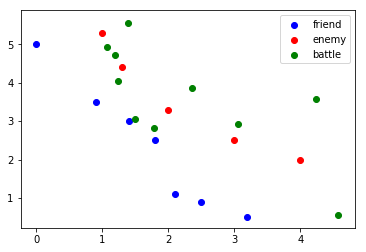
\includegraphics[width=0.6\linewidth]{exp_state.png}
\caption{Given situation}
\label{fig:expState}
\end{figure}


\subsubsection{MAP}

Firstly, if flat prior is used (only provide likelihood), the MAP result is Figure~\ref{fig:MAPone}.

\begin{figure}[h]
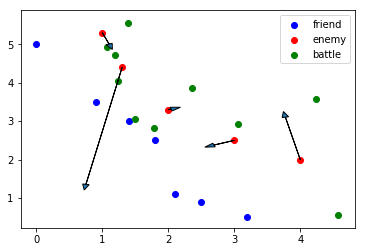
\includegraphics[width=0.6\linewidth]{MAP1.png}
\caption{MAP with flat prior}
\label{fig:MAPone}
\end{figure}

The arrowtail indicate the "true" position of enemy(though it can't be seen), 
the arrowhead indicate the estimated position of enemy for MAP. As we can see,
a enemy is pulled to the back of ally units to maximize probability, it seems overfit anyway.
We can utilize the advatage of bayes framework, adding a prior \footnote{Or regulation term, but I
prefer the probability meaning offered by bayes.}:


$$
P_{\text{enemy}}(x,y) = \exp(sig(t((x+y) - \alpha)))
$$

Where $t$ is tense parameter for enemy position,
$\alpha$ is corresponding threshold. We set $t=5.0,\alpha=5.0$
for illustration below.

The new joint probability with the diagonal prior is:

\begin{align*}
\log p(\mathbf{x}^E,\mathbf{y}^E) &= \sum_{i=1}^B \log sig(t (P_\text{ally}(x^B_i,y^B_i)(1-P_\text{ally}(x^B_i,y^B_i)) - \theta_0)) \\
                                  &+ \sum_{i=1}^B \log sig(t(-\min_{u} distance(x^B_i,y^B_i) + \theta_1)) \\
                                  &+ \sum_{j=1}^E sig(t((x^E_j+y^E_j) - \alpha))
\end{align*}

Where $B,E$ are number of battle and enemy,$x^B_i,y^B_i$ is coordinate of battle $i$, $x^E_j,y^E_j$
is coordinate of enemy $j$.

The result of MAP on the new probability function looks better as shown in the Figure~\ref{fig:MAPtwo}.

\begin{figure}[h]
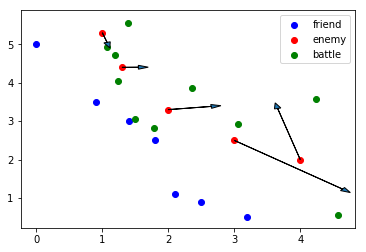
\includegraphics[width=0.6\linewidth]{MAP2.png}
\caption{MAP with diagonal prior}
\label{fig:MAPtwo}
\end{figure}

\subsubsection{Sampling and Variational inference}

Point estimation is not enough since it can't give uncertain information about the estimation.
Tough exact posterior may fix it but it's hard to compute and represent. Two ways in bayes inference 
to do it are sampling and variational inference(VI). The former one generate a "trace" which can be thought
as a sample taken from exact posterior, the trace may contitude empirical distribution or reveal 
attribution of the random parameter. The VI is faster but lack exact attribution.

The two results of VI in flat prior and new diagonal prior can be seen in Figure~\ref{fig:VI}.
The two results of sampling can be seen in Figure~\ref{fig:samping}.

\begin{figure}[h]
  \begin{subfigure}[b]{0.45\linewidth}
    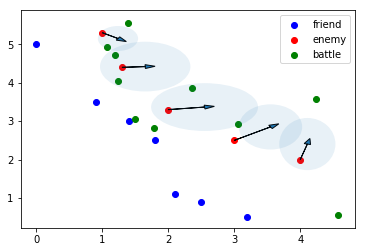
\includegraphics[width=\linewidth]{VI11.png}
    \caption{VI with flat prior A}
  \end{subfigure}
  \begin{subfigure}[b]{0.45\linewidth}
    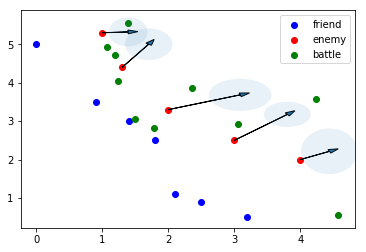
\includegraphics[width=\linewidth]{VI12.png}
    \caption{VI with diagonal prior A}
  \end{subfigure}
  \begin{subfigure}[b]{0.45\linewidth}
    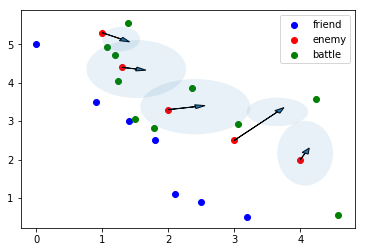
\includegraphics[width=\linewidth]{VI21.png}
    \caption{VI with flat prior B}
  \end{subfigure}
  \begin{subfigure}[b]{0.45\linewidth}
    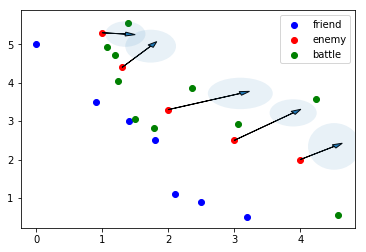
\includegraphics[width=\linewidth]{VI22.png}
    \caption{VI with diagonal prior B}
  \end{subfigure}
  \caption{VI fit result}
  \label{fig:VI}
\end{figure}

\begin{figure}[h]
  \begin{subfigure}[b]{0.45\linewidth}
    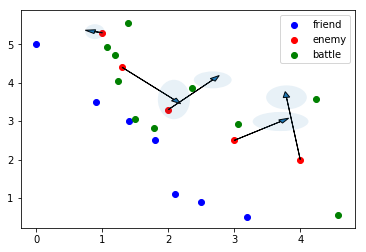
\includegraphics[width=\linewidth]{Sampling11.png}
    \caption{HMC with flat prior A}
  \end{subfigure}
  \begin{subfigure}[b]{0.45\linewidth}
    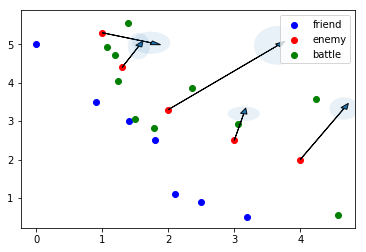
\includegraphics[width=\linewidth]{Sampling12.png}
    \caption{HMC with diagonal prior A}
  \end{subfigure}
  \begin{subfigure}[b]{0.45\linewidth}
    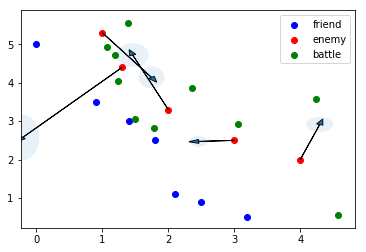
\includegraphics[width=\linewidth]{Sampling21.png}
    \caption{HMC with flat prior B}
  \end{subfigure}
  \begin{subfigure}[b]{0.45\linewidth}
    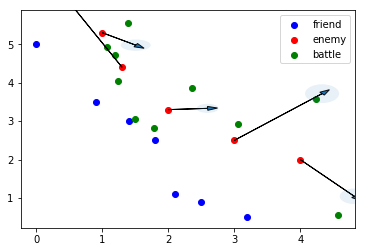
\includegraphics[width=\linewidth]{Sampling22.png}
    \caption{HMC with diagonal prior B}
  \end{subfigure}
  \caption{samping fit result(100 samples)}
  \label{fig:samping}
\end{figure}

Where the coordinate of ellipses indicate the expectation of those posterior distribution,
and the radius of ellipses indicate the standard deviation(sd) of axis x and y in every latent enemy point.
So those ellipse can be seen as a rough approximation for posterior distribution 
hidden in trace or variational distribution, though those two are not exact posterior too.

The HMC result seems inconsisitency, implying the converge fail. Though increasing sample size may be
solution(see Figure~\ref{fig:SamplingTen}). But just like we are not content to a NP-hard solver and claim that it only need more time,
sampling seems too weak in this problem.

\begin{figure}[h]
  \begin{subfigure}[b]{0.45\linewidth}
    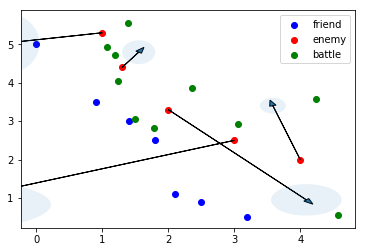
\includegraphics[width=\linewidth]{Sampling31.png}
    \caption{HMC with flat prior A}
  \end{subfigure}
  \begin{subfigure}[b]{0.45\linewidth}
    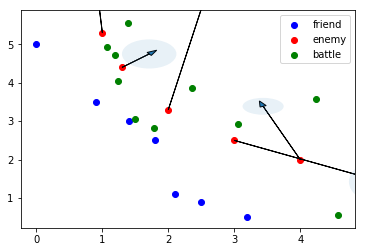
\includegraphics[width=\linewidth]{Sampling32.png}
    \caption{HMC with diagonal prior A}
  \end{subfigure}
  \begin{subfigure}[b]{0.45\linewidth}
    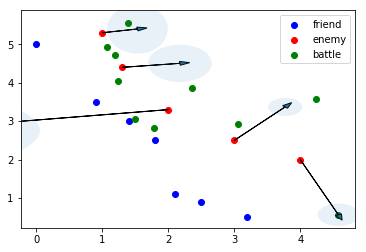
\includegraphics[width=\linewidth]{Sampling41.png}
    \caption{HMC with flat prior B}
  \end{subfigure}
  \begin{subfigure}[b]{0.45\linewidth}
    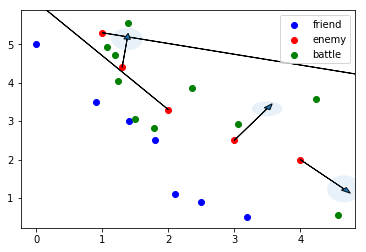
\includegraphics[width=\linewidth]{Sampling42.png}
    \caption{HMC with diagonal prior B}
  \end{subfigure}
  \caption{samping fit result(1000 samples)}
  \label{fig:SamplingTen}
\end{figure}

\subsection{Mutiple enemy number setting}

The above estimation is based on "true" number of enemy. Let we test it's stability. 
What happen if the given number of number of enemy is wrong? The Figure~\ref{fig:bigVb} 
show the result, that flat prior seems well while diagonal prior may may be dominated by 
the prior. But it depict what we want in general.

\begin{figure}[h]
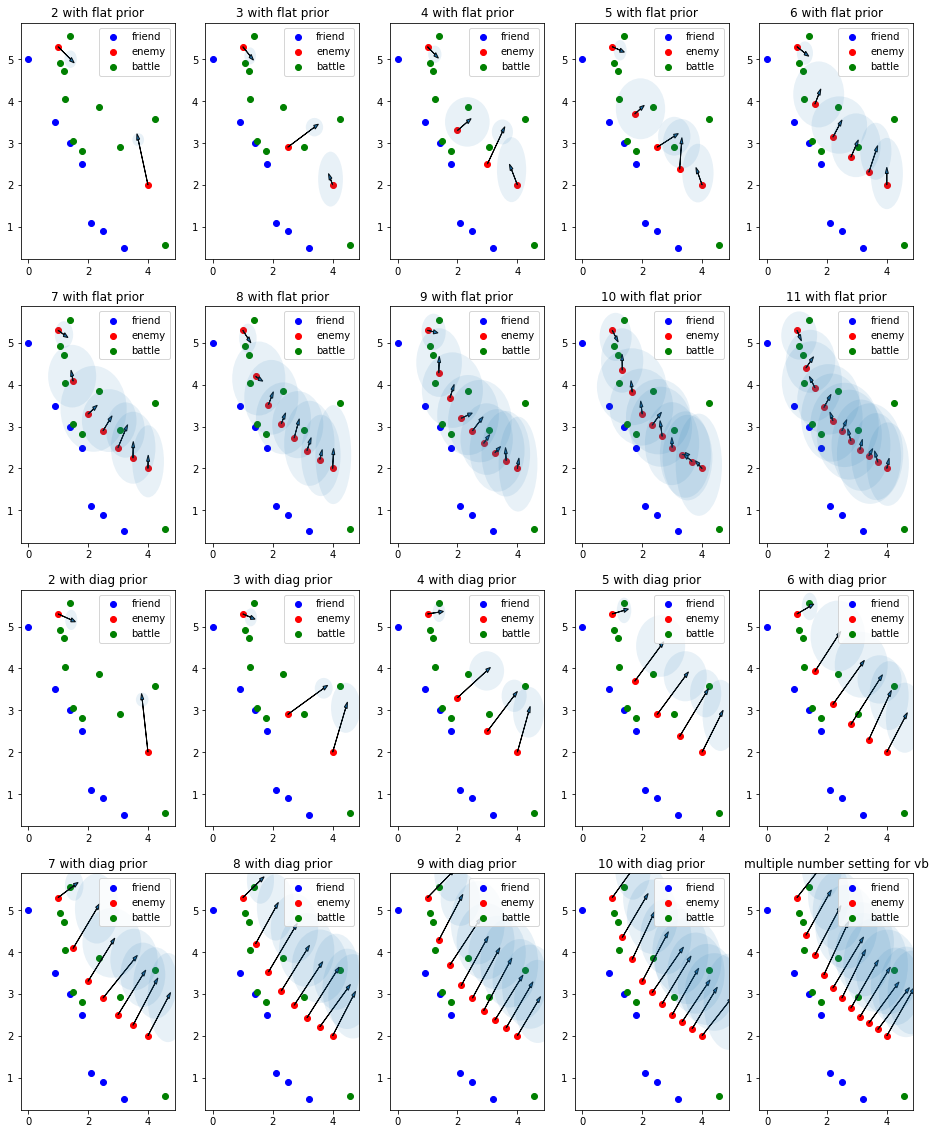
\includegraphics[width=0.99\linewidth]{big_vb.png}
\caption{Mutiple setting for approximation}
\label{fig:bigVb}
\end{figure}

\subsubsection{The density of probabity of existence of enemy estimation}

The one of advantage of VB is that it make computation of probability of special region very easy.
The probability of exist of enemy in a given region $[x,x+dx]\times[y,y+dy]$ can be given by:

$$
pe(x,y,dx,dy) = 1 - \prod_i \left(
(1-(\Phi(x+dx - \mu^X_i)/\sigma^X_i) -  (\Phi(x - \mu^X_i)/\sigma^X_i))
(1-(\Phi(y+dy - \mu^Y_i)/\sigma^Y_i) -  (\Phi(y - \mu^Y_i)/\sigma^Y_i))
\right)
$$

Where $\Phi(x)$ is standard cumulative probability function:

$$
\Phi(x) = \int_{-\infty}^x \frac{1}{\sqrt{2\pi}} \exp\left(\frac{x^2}{2}\right)
$$

And $$\mu^X_i$$ is the expect parameter of normal approximated posterior probability of ith enemy.
The three other are same.

The existence density(approximated) is defined:

$$
pe(x,y) = pe(x-\epsilon,y-\epsilon,2\epsilon,2\epsilon)/(4*\epsilon^2)
$$

Where $\epsilon$ is a small number, in there $\epsilon=0.01$. 
The two example can be seen in Figure~\ref{fig:existDensity}. 
The comparing result can be seen in seen in Figure~\ref{fig:bigVbExist}.

\begin{figure}[h]
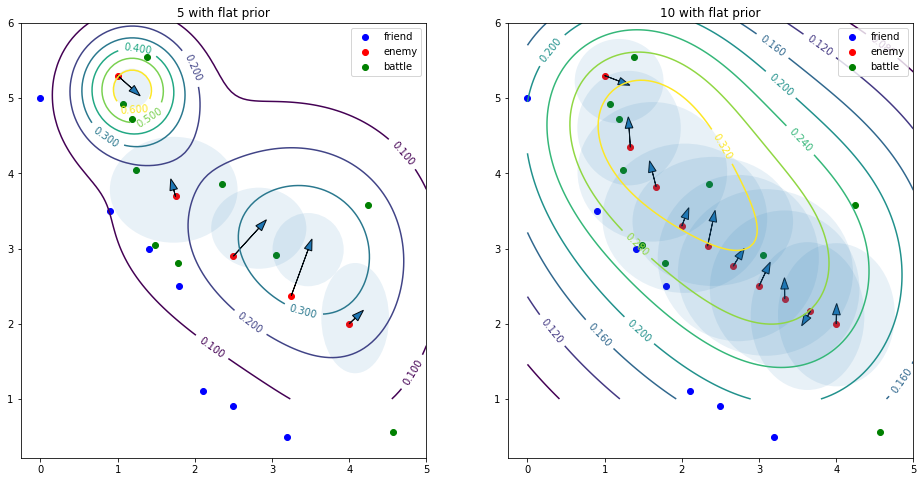
\includegraphics[width=0.99\linewidth]{exist_density.png}
\caption{Two enlarged exist density situation}
\label{fig:existDensity}
\end{figure}


\begin{figure}[h]
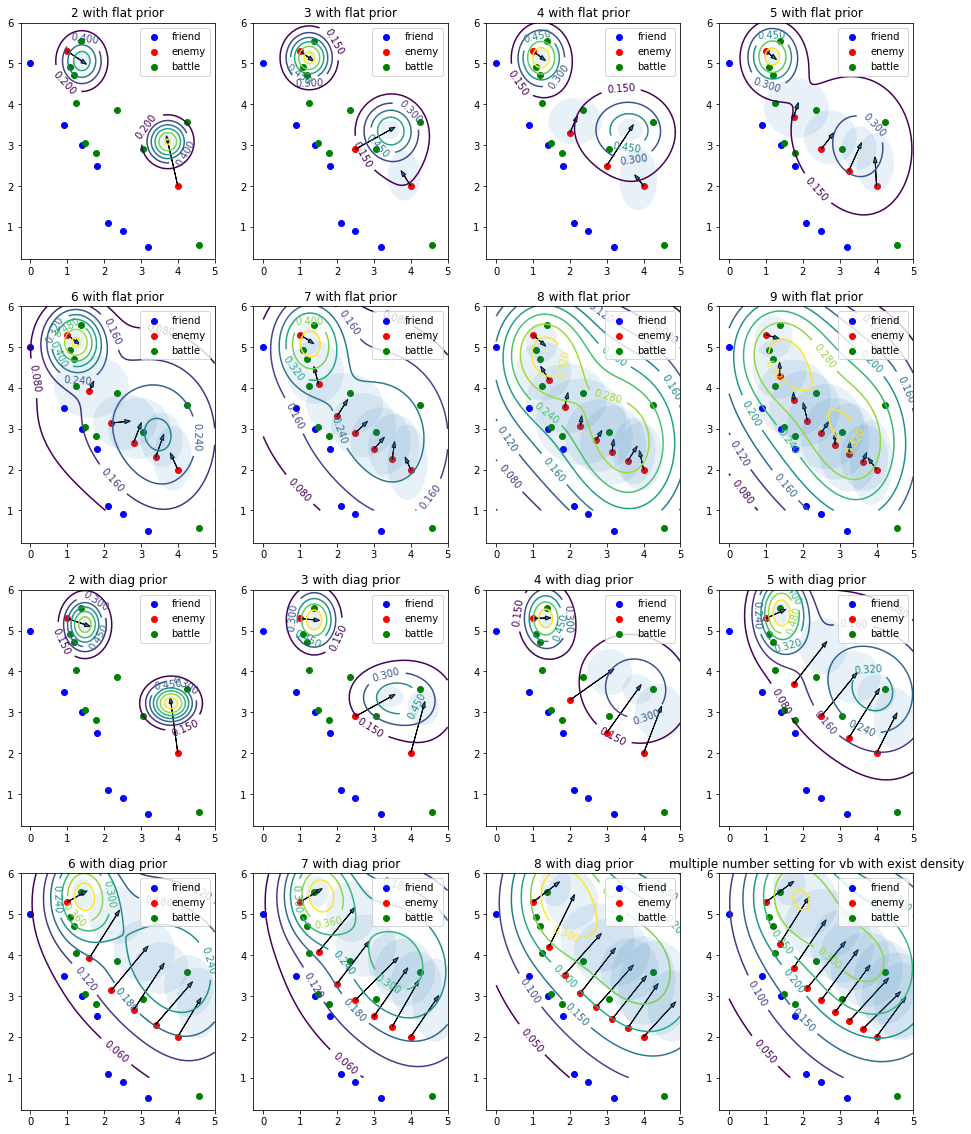
\includegraphics[width=0.99\linewidth]{big_vb_exist_prob.png}
\caption{Mutiple setting fit with exist probabiliy}
\label{fig:bigVbExist}
\end{figure}



\section{Extention: Enemy movement detecting}

Considering ally,enemy,battles have not only position, but also have timestamp. In another word,
enemy and ally may move in the time, how do we infer the movement?

Interestingly, the model only need a little modification to integrate the setting.

Assurming the time begin at $0$ and end at $1$, and enemy have uniform motion in constant speed.
So the parameters$x^E_i$ can be rewritten as $x^E_i(t) = (1-t)x^E_i(0) + tx^E_i(1)$, 
$x^E_i(0),x^E_i(1)$ means the position of ith enemy in time 0 and 1 respectively, and so on.
They are new parameters. The other structual probability function almost keep its original form.

First, assurming $x^E_i(0),y^E_i(0)$ are known and $x^E_i(1),y^E_i(1)$ are unknown.
A instance of inference shown in Figure~\ref{fig:bkeu}. Where arrowtail indicate the known begin point.
The one of two arrowhead surrounded by sd ellipse is estimated $t=1$ coordination expectation. 
The another is "true" point.

\begin{figure}[h]
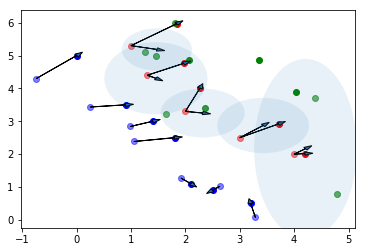
\includegraphics[width=0.4\linewidth]{bkeu.png}
\caption{The $t=0$ situation known but $t=1$ not}
\label{fig:bkeu}
\end{figure}

The following Figure~\ref{fig:bueu} show the situation in which $t=0,1$ situation are both unknown
\footnote{Note they're not in same data set.}. Where the arrowtail of first arrow is "true" begin
point, the middile point is estimated posterior expect of the point at $t=0$, the arrowhead of second arrow
is estimated posterior expect of the point at $t=1$.

\begin{figure}[h]
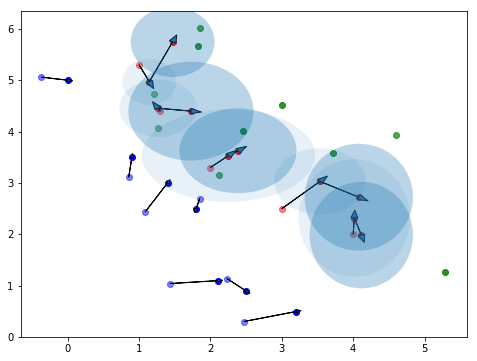
\includegraphics[width=0.6\linewidth]{bueu.png}
\caption{Both $t=0$ situation and $t=1$ are unknown}
\label{fig:bueu}
\end{figure}

The prior that give punishment to too long moving range also are useful and easy to implement. 
But the dataset that can highlight the advantage don't be constructed yet subject to time limit.
So it will be skiped.

\section{Extention: Dealing complex position distribution.}

The above content is based on similar distribution, a curve can divide ally and enemy easily.
What will happen if the shape become complex and hard to capture for "one center" bayes naive classifer?

\subsection{Circle}

The "true" position is droped. This section will contain only "initialization value"
(In above content, "true position" play also initialization value role.). 
The Figure~\ref{fig:circleIteration} show the circle setting with flat prior, 
showing also a nice iteration convege process .


\begin{figure}[h]
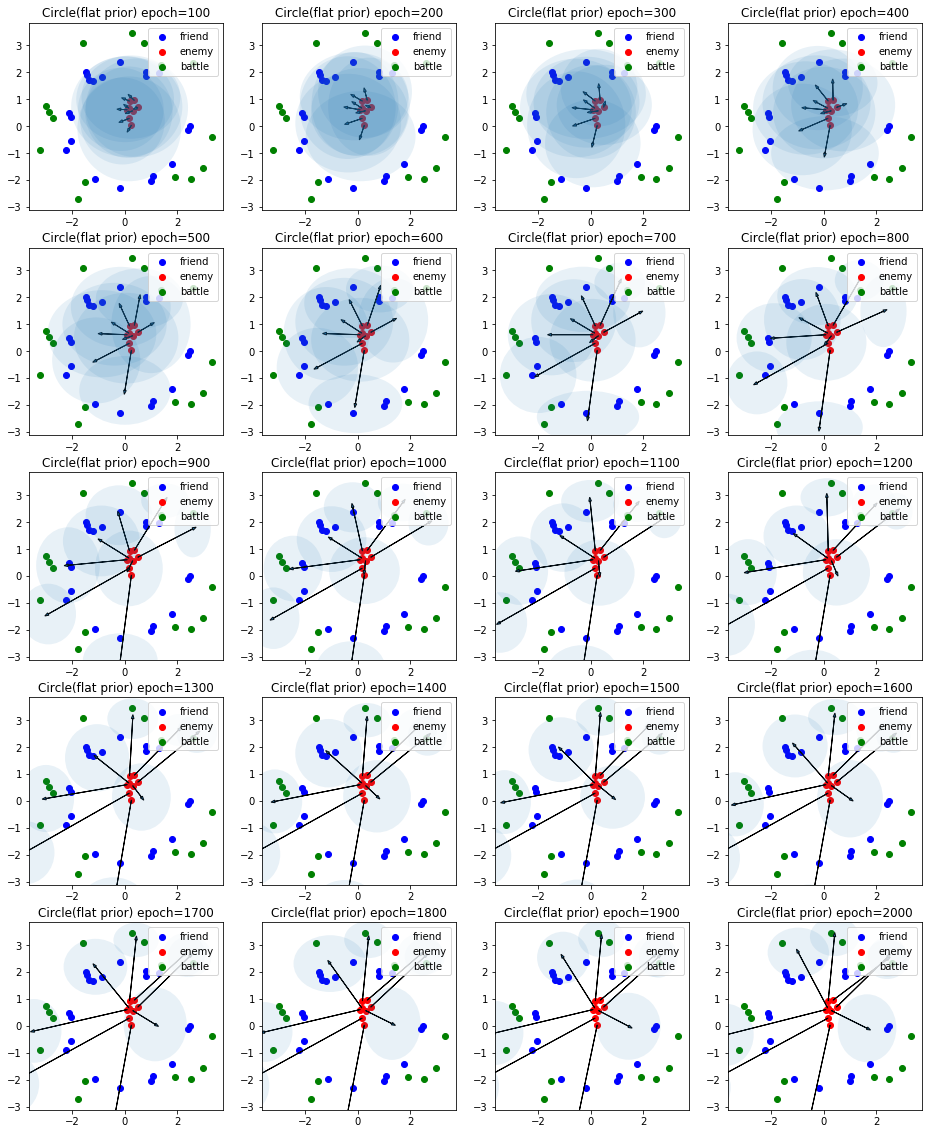
\includegraphics[width=0.99\linewidth]{circle_iteration.png}
\caption{Iteration process for circle setting with flat prior and random initialization}
\label{fig:circleIteration}
\end{figure}

\subsection{Case study: The battle of Gettysburg}

Now, it's the time to abandon the globular chicken in vacuum loved by physicists.
The Figure~\ref{fig:gettysburg} show the map and data of the battle of Gettysburg in second day.
The data only capture the division(NATO:XX)  in the map.
The confederate have less number of division since the size of the division of CSA are more big.
The data is from HPS great wargame "Civil war:Gettysburg". 
The data used listed in the Table~\ref{tab:Confederate} and \ref{tab:Union}, in which strength 
is number of unit that is not used in the model yet and will be used in later section as weight.

\begin{table}
\parbox{.45\linewidth}{
\begin{tabular}{lrrr}
\toprule
{} &  strength &    x &    y \\
\midrule
Heth's Div     &      4628 &  2.4 &  4.8 \\
McLaws' Div    &      6762 &  2.9 &  1.0 \\
Hood's Div     &      6957 &  3.3 &  0.1 \\
Anderson's Div &      6686 &  3.5 &  2.8 \\
Pender's Div   &      5080 &  3.6 &  3.7 \\
Rodes' Div     &      5202 &  5.0 &  4.2 \\
Early's Div    &      4572 &  6.0 &  3.9 \\
Johnson's Div  &      6012 &  7.2 &  4.5 \\
\bottomrule
\end{tabular}
\caption{Confederate oob}
\label{tab:Confederate}
}
\hfill
\parbox{.45\linewidth}{
\begin{tabular}{lrrr}
\toprule
{} &  strength &    x &    y \\
\midrule
2nd D (Humphreys)   &      4913 &  4.2 &  1.7 \\
1st Div (Birney)    &      5008 &  4.5 &  0.8 \\
2nd Div (Gibbon)    &      3558 &  5.1 &  2.3 \\
3rd Div (Hays)      &      3622 &  5.2 &  2.6 \\
1st Div (Caldwell)  &      3303 &  5.2 &  1.8 \\
3rd Div (Schurz)    &      1633 &  5.3 &  3.1 \\
2nd Div (Steinwehr) &      2264 &  5.4 &  2.9 \\
3rd Div (Doubleday) &      2922 &  5.4 &  2.7 \\
1st Div (Barlow)    &      1475 &  5.5 &  3.1 \\
2nd Div (Robinson)  &      1311 &  5.5 &  2.6 \\
1st Div (Wadsworth) &      1697 &  6.2 &  3.0 \\
2nd Div (Geary)     &      3851 &  6.2 &  2.8 \\
1st Div (Williams)  &      4698 &  6.3 &  2.1 \\
2nd Div (Ayres)     &      3990 &  6.6 &  1.6 \\
1st Div (Barnes)    &      3411 &  6.7 &  1.7 \\
3rd Div (Crawford)  &      2842 &  6.8 &  1.6 \\
3rd Div (Newton)    &      4729 &  7.3 &  0.8 \\
1st Div (Wright)    &      4181 &  7.4 &  1.2 \\
2nd Div (Howe)      &      3548 &  9.3 &  0.0 \\
\bottomrule
\end{tabular}
\caption{Union oob}
\label{tab:Union}
}
\end{table}

Following we assurm the position of army of Union and battle are known but CSA not.

\begin{figure}[h]
  \begin{subfigure}[b]{0.49\linewidth}
    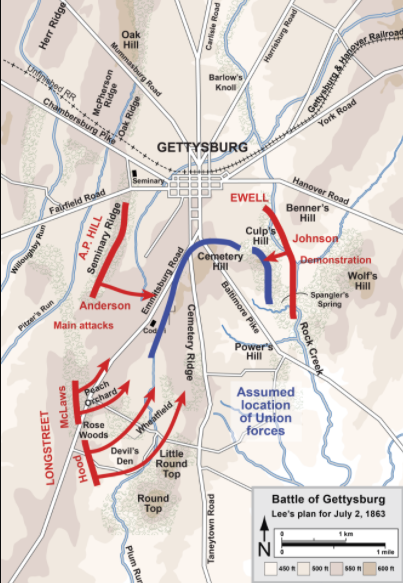
\includegraphics[width=\linewidth]{gettysburg-map.png}
    \caption{Map of battle of Gettysburg, second day}
  \end{subfigure}
  \begin{subfigure}[b]{0.49\linewidth}
    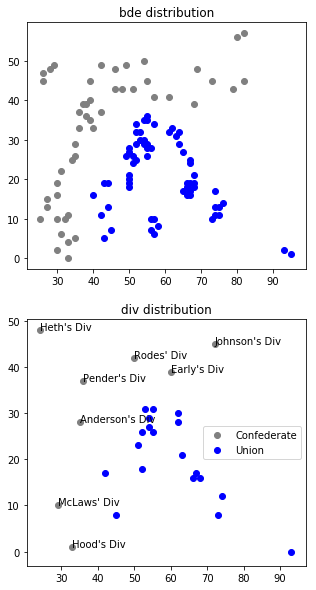
\includegraphics[width=\linewidth]{gettysburg-model.png}
    \caption{Simple model for the situation}
  \end{subfigure}
  \caption{Comparing between real and model setting}
  \label{fig:gettysburg}
\end{figure}

In Figure~\ref{fig:gettysburgTwo} the forward probability model is illustrated and a sample of the model and observed
ally unit.

\begin{figure}[h]
  \begin{subfigure}[b]{0.49\linewidth}
    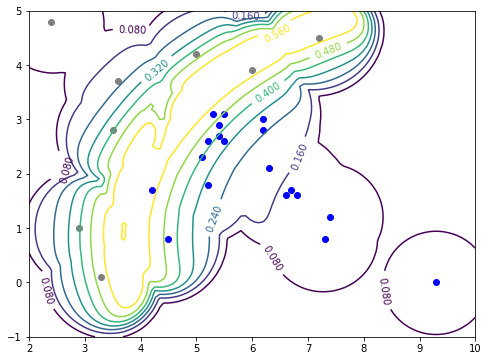
\includegraphics[width=\linewidth]{gettysburg-forward.png}
    \caption{Unnormalized probability of battle occuring}
  \end{subfigure}
  \begin{subfigure}[b]{0.49\linewidth}
    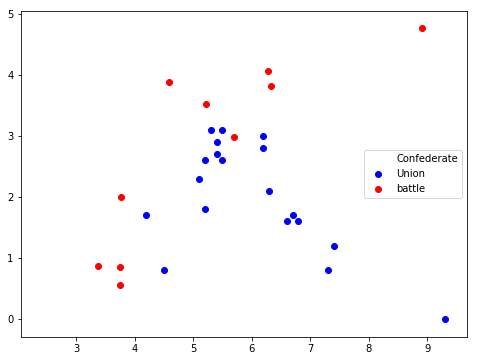
\includegraphics[width=\linewidth]{gettysburg-sample.png}
    \caption{A sample of occuring battle and ally unit.}
  \end{subfigure}
  \caption{The forward model and a sample of it}
  \label{fig:gettysburgTwo}
\end{figure}

We can run procedure described above with randomized initialized point. 
Figure~\ref{fig:gettysburgInit} show the exist-probability and converge process.

\begin{figure}[h]
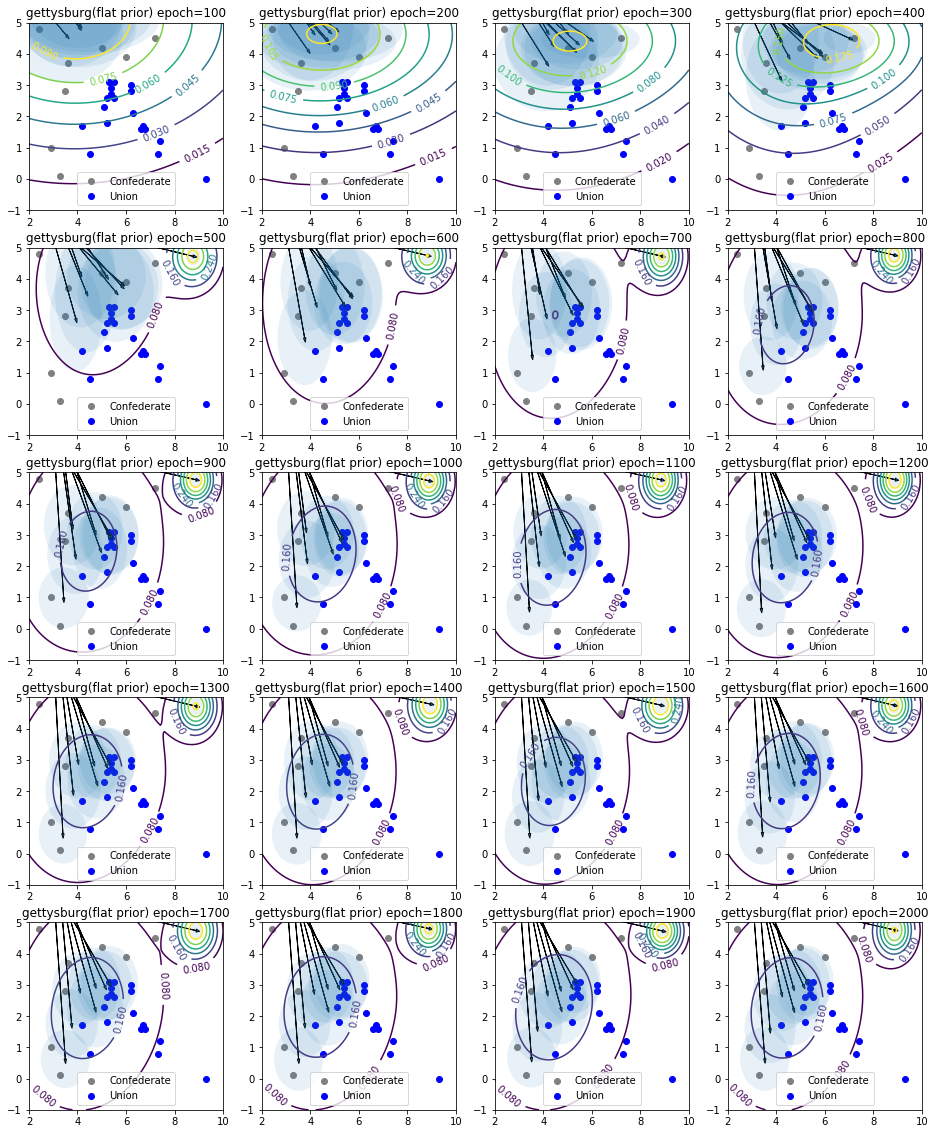
\includegraphics[width=0.99\linewidth]{gettysburg-init.png}
\caption{Iteration process for randomized initialized setting with flat prior in Gettysburg sample}
\label{fig:gettysburgInit}
\end{figure}

It looks good, thougn the enemy units seems too close to ally. It can be solved a bit by prior.


\section{Extention: Size effect}

The above content assurm battles and units are homogeneous. It may make sense,
but if battle and unit can include number and size information, the result will be more useful.

To extend our model to embrace the change, we can merely define the high weight the unit have,
the long radius in distance factor and large weight in estimation on center of class unit cause.

Following content use the strength of Table~\ref{tab:Confederate} and \ref{tab:Union} as weight.
The $\mu,\sigma$ used by naive bayes classifer is computed by weithted version now.
And the distance will be adujusted to $dist_{ij} = dist_{ij} \frac{\beta}{stre_i}$, the $\beta$
is seted to $6000$. So all of units of Union will be penalized, 
and a few of Confederate will be bonused for distance factor.

The Figure~\ref{fig:gettysburgInitTwo} show the result, it very like the result fited without size effect. 
It turn out that the model is steady for suct effect.

\begin{figure}[h]
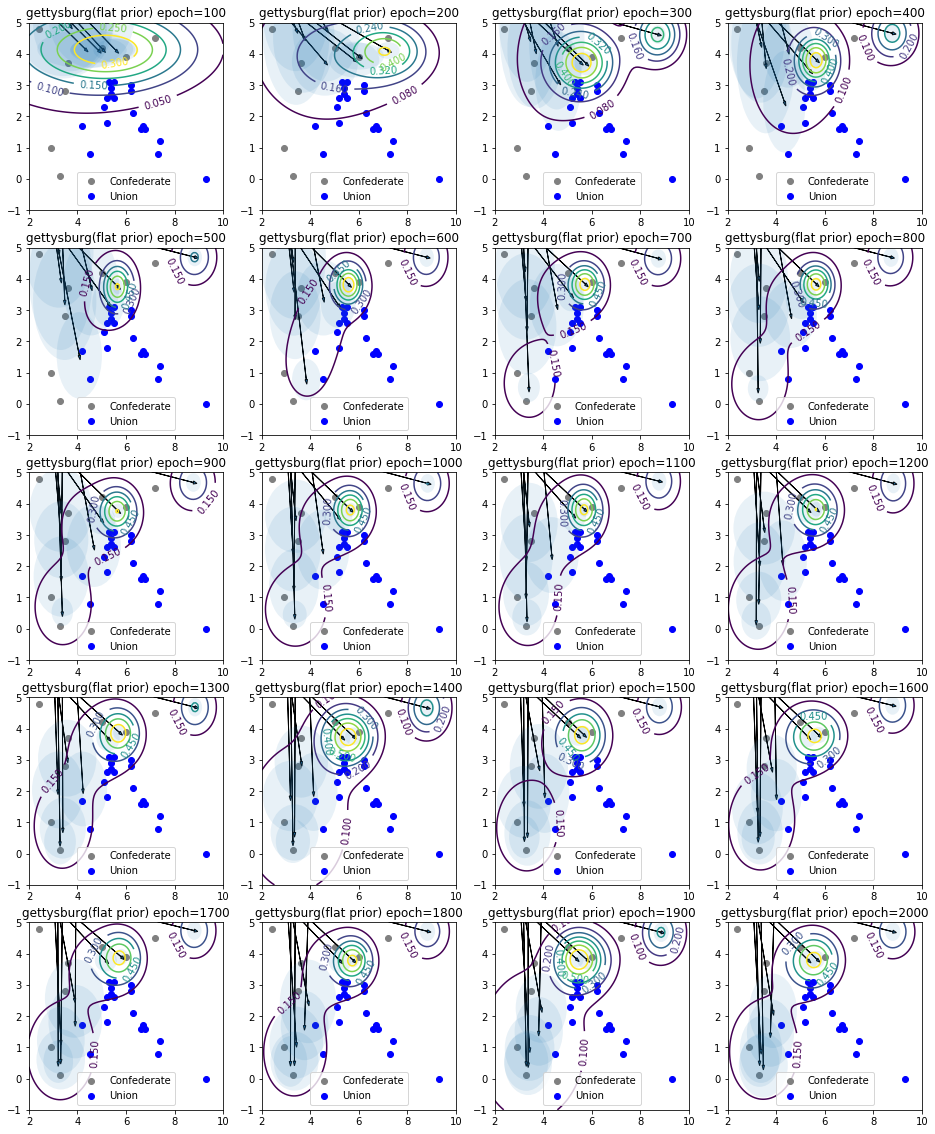
\includegraphics[width=0.99\linewidth]{gettysburg-init2.png}
\caption{Iteration process for randomized initialized setting with flat prior with Size effect}
\label{fig:gettysburgInitTwo}
\end{figure}


\section{Conclusion}

We present a standard bayes inference framework 
\footnote{In fact, the content of the paper have been implmented as examples of a open-source library
hosted in GitHub, see: \url{https://github.com/yiyuezhuo/bayes-torch} where yiyuezhuo is the nickname of
the writer Yueyi Zhuo} 
in a classes of prolbem in which 
two class of point(ally and enemy) will generate another class of points(battle), 
when one class is hidden(enemy).

The forward model can transformed easily to backward model to do inference due to our framework.
The inference include point detection, movement dectection with prior or adujusted prior.
They're be checked its steady and converge performance by true initialization and random initialization.
A case study about battle of Gettysburg summary the content covered by the paper. 
I wish the result can be producation environment and my game designing.

Designing the forward model, doing its inference and balancing effciency and correctness 
are interesting challenge, but useful.

\bibliography{paper} 
\bibliographystyle{ieeetr}

\end{document}